\documentclass[../250428_msquare_provable_security.tex]{subfiles}

\begin{document}

\subsection{PRP/PRF Switching}
\begin{frame}{Motivation}
    \begin{center}
        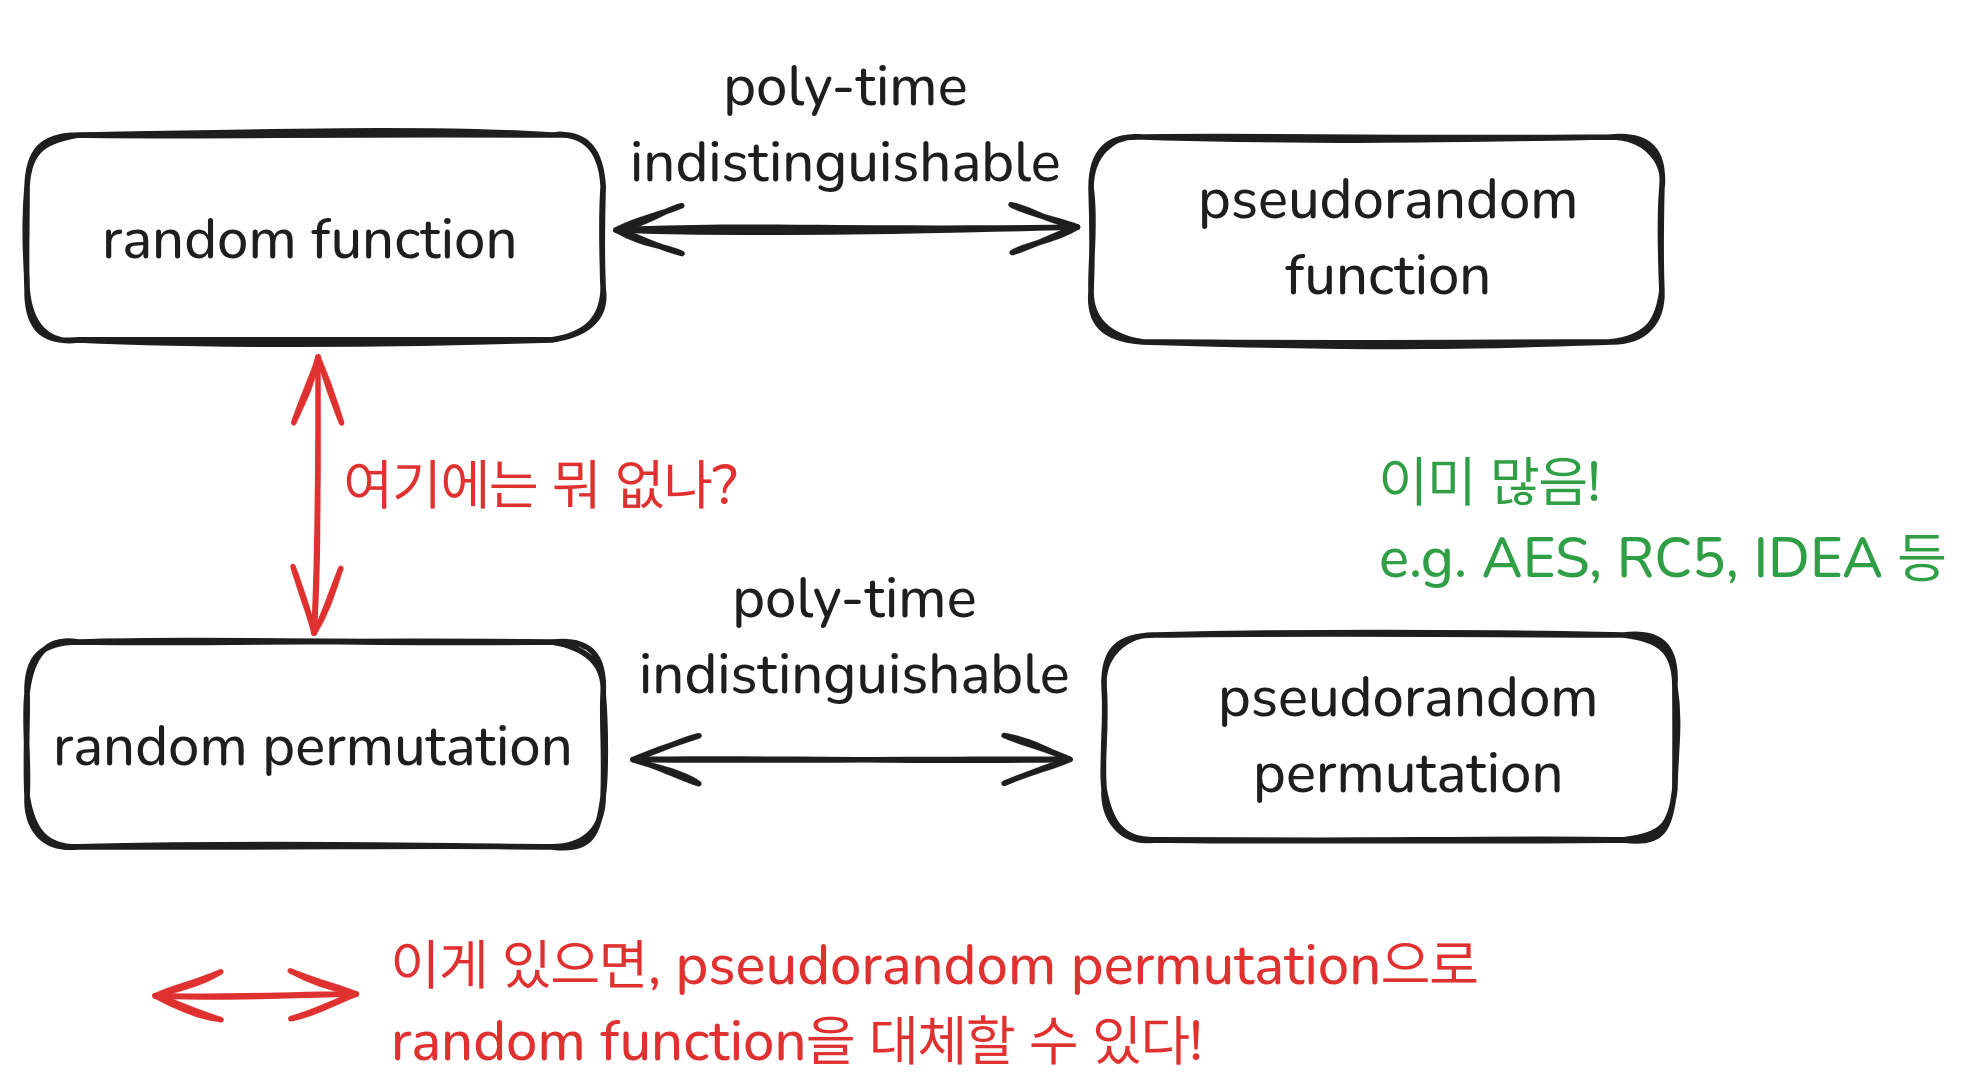
\includegraphics[width=.9\textwidth]{../switching_motivation.png}
    \end{center}
\end{frame}

\begin{frame}{The Security Game}
    어떤 방어자와 (시간이 무제한인) 어떤 probabilistic algorithm \(\mcal{D}\)가 공격자인
    다음 security game을 생각해 보자.
    \pause
    \begin{enumerate}
        \ii
        방어자는 \(b \in \{0,1\}\)를 uniform하게 고른다.
        \pause
        \ii
        \(b = 0\)이면, 방어자는
        임의의 \(f^\ast \gets \mcal{P}_n\)을 고른다.
        \ii
        \(b = 1\)이면, 방어자는
        임의의 \(f^\ast \gets \mcal{F}_n\)을 고른다.
        \pause
        \ii
        공격자는 여러 번의 ``질의''를 할 수 있다.
        각 질의 \(x_i\)에 대해 방어자는 \(y_i = f^\ast(x_i)\)를 공격자에게 알려준다.
        \pause
        \ii
        모든 질의의 마지막에 공격자는 \(b' \in \{0,1\}\)을 결정한다.
        만약 \(b = b'\)이면 공격자가 이기고, \(b \neq b'\)이면 방어자가 이긴다.
    \end{enumerate}
\end{frame}

\begin{frame}{The Security Game}
    \begin{block}{Advantage of Distinguisher}
        \begin{itemize}
            \ii
            공격자 \(\mcal{D}\)에 대해,
            \begin{align*}
                P_{\msf{re}} &\coloneqq \Pr[P \dgets \mcal{P}_n \colon 1 \gets \mcal{D}^{P}] \\
                P_{\msf{id}} &\coloneqq \Pr[F \dgets \mcal{F}_n \colon 1 \gets \mcal{D}^{F}]
            \end{align*}
            이라고 하면,
            \[
                \msf{Adv}(\mcal{D}) = |P_{\msf{id}} - P_{\msf{re}}|
            \]
            라고 하자.
            \ii
            질의를 최대 \(q\)번 하는 \(\mcal{D}\)의 최대 \(\msf{Adv}(\mcal{D})\)값을
            \(\msf{Adv}(q)\)라고 하자.
            \end{itemize}
    \end{block}

\end{frame}

\begin{frame}{PRP/PRF Switching Lemma}
    \begin{block}{PRP/PRF Switching Lemma}
        \[
            \msf{Adv}(q) \le \frac{q^2}{2^n}\text.
        \]
    \end{block}

    뜻?
\end{frame}

\subsection{Proof}
\begin{frame}{Assumptions}
    우리는 다음을 가정할 수 있다.
    \pause
    \begin{enumerate}
        \ii \(\mcal{D}\)는 중복된 질의를 하지 않는다.
        \pause
        \ii \(P_{\msf{id}} \ge P_{\msf{re}}\)
        \pause
        \ii \(\mcal{D}\)는 ``동전을 던지지 않는다''. (probabilistic choice를 하지 않는다.)
    \end{enumerate}
\end{frame}

\begin{frame}{Transcripts}
    \begin{block}{Transcript}
        \(\mcal{D}\)가 \(q\)회의 질의
        \(x_1, \cdots, x_q\)를 하면,
        답변 \(y_1, \cdots, y_q\)를 얻는다.
        이런 tuple
        \[
            (x_1, x_2, \cdots, x_q, y_1, y_2, \cdots, y_q)
        \]
        를 transcript라고 부르고, transcript의 집합을 \(\mcal{T}\)라고 하자.
    \end{block}
    \pause

    \begin{alertblock}{}
        \(\mcal{D}\)가 동전을 던지지 않기 때문에,
        \(\mcal{D}\)의 출력은 \(\mcal{D}\)가 가진 transciprt \(\tau \in \mcal{T}\)에 의해서 결정된다!
    \end{alertblock}
\end{frame}

\begin{frame}{Transcripts}
    \(T_{\msf{re}}\), \(T_{\msf{id}}\)를 \(\mcal{T}\) 위의 다음과 같은 확률 변수라고 하자.
    \begin{itemize}
        \ii
        \(\Pr[T_{\msf{re}} = \tau] = \mbox{}\)\(\mcal{D}\)가 real world에서 \(\tau\)를 얻을 확률
        \ii
        \(\Pr[T_{\msf{id}} = \tau] = \mbox{}\)\(\mcal{D}\)가 ideal world에서 \(\tau\)를 얻을 확률
    \end{itemize}

    \pause
    그러면,
    \begin{align*}
        P_{\msf{re}} &= \Pr[P \dgets \mcal{P}_n \colon 1 \gets \mcal{D}^{P}]
        = \sum_{\tau \colon \mcal{D}(\tau) \to 1} \Pr[T_{\msf{re}} = \tau] \\
        P_{\msf{id}} &= \Pr[F \dgets \mcal{F}_n \colon 1 \gets \mcal{D}^{F}]
        = \sum_{\tau \colon \mcal{D}(\tau) \to 1} \Pr[T_{\msf{id}} = \tau]\text,
    \end{align*}
    \pause
    즉
    \[
        \msf{Adv}(\mcal{D})
        = \sum_{\tau \colon \mcal{D}(\tau) \to 1} (\Pr[T_{\msf{id}} = \tau] - \Pr[T_{\msf{re}} = \tau])\text.
    \]
\end{frame}

% \begin{frame}{Transcripts}
%     \begin{center}
%         \includegraphics[width=.8\textwidth]{../transcript1.png}
%     \end{center}
% \end{frame}
%
% \begin{frame}{Transcripts}
%     \begin{center}
%         \includegraphics[width=.8\textwidth]{../transcript2.png}
%     \end{center}
% \end{frame}

\begin{frame}{Transcripts}
    따라서
    \begin{align*}
        \msf{Adv}(\mcal{D})
        &= \sum_{\tau \colon \mcal{D}(\tau) \to 1} (\Pr[T_{\msf{id}} = \tau] - \Pr[T_{\msf{re}} = \tau]) \\
        &\le \sum_{\tau \colon \Pr[T_{\msf{id}} = \tau] > \Pr[T_{\msf{re}} = \tau]} (\Pr[T_{\msf{id}} = \tau] - \Pr[T_{\msf{re}} = \tau]) \\
        &\le \sum_{\tau\text{ has duplicate outputs}} (\Pr[T_{\msf{id}} = \tau] - \Pr[T_{\msf{re}} = \tau]) \\
        &\le \sum_{\tau\text{ has duplicate outputs}} \Pr[T_{\msf{id}} = \tau] \\
        &\le \binom{q}{2}\frac{1}{2^n} \le \frac{q^2}{2^{n+1}}\text.
    \end{align*}
\end{frame}

\end{document}
